\chapter{Wariancja Allana}\label{chap:appx:allan}
Wariancja Allana jest metodą wykorzystywaną do określenia charakterystyk szumów zawartych w~sygnałach mierzonych przez układy oparte o~oscylatory. Metoda ta została opisana w~\cite{Allan1966} jako część pracy magisterskiej w~latach 60-tych XX wieku i~od tamtego czasu została przyjęta jako standardowa do wyznaczania charakterystyk tego typu układów. W~literaturze można znaleźć między innymi prace opisujące analizę sygnałów układów inercyjnych \cite{El-Sheimy2008, FreescaleSemiconductor2015}, czy układów GPS \cite{Wright2007}. 
Wariancja Allana ($\sigma_{\Omega}^2(t)$) wyznaczana jest dla sygnału $\Omega$ wyrażonego w~domenie czasu i~podzielonego na $N$ przedziałów o~czasie trwania $t$ każdy. Przyjmując, że $n$ oznacza numer klastra badanego sygnału, a $\Omega_n(t)$ oznacza wartość sygnału w przedziale o numerze $n$, wariancję Allana możemy wyrazić za pomocą równania \ref{eq:appx:allan:avar}\cite{Sochocka2004}.

\begin{equation}
	\label{eq:appx:allan:avar}
	\sigma_{\Omega}^2(t) = \frac{1}{2(N-1)}\sum[\Omega_{n+1}(\tau)-\Omega_n(\tau)]^2
\end{equation}

		
Aby na podstawie wyznaczonej wariancji określić charakterystyki szumów należy obliczyć odchylenie Allana $\sigma_{\Omega}(t) = \sqrt{\sigma^2(t)}$ i~przeanalizować przebieg tej funkcji na wykresie w~skali logarytmicznej (przykładowy wykres odchylania Allana dla żyroskopu przedstawia wykres z rysunku \ref{fig:appx:allan:slopes}). Wykres ten zawiera informacje o~5 różnych rodzajach szumu jakie są zawarte w~badanym sygnale (nazwy szumów na podstawie \cite{PASZEK2016}):
		
\begin{enumerate}
	\item {Błąd kwantyzacji -- szum wprowadzony w~trakcie konwersji sygnału analogowego na cyfrowy i~spowodowany przez różnice pomiędzy faktyczną wartością sygnału, a~wartością wynikającą z~punktu, w~którym nastąpiło próbkowanie.}
	\item {Błąd ARW -- szum wysokiej częstotliwości obserwowalny nawet w~czasie krótkich pomiarów. Jego występowanie znacząco obniża dokładność prowadzonych obliczeń.}
	\item {Bład BI -- szum niskiej częstotliwości związany ze zmianą właściwości fizycznych materiałów, z~których zbudowane są czujniki, a~przez to niepoprawną interpretacją napięcia elektrycznego działającego w~urządzeniu.}
	\item {Błąd RRW -- szum wysokiej częstotliwości pojawiający się w~pomiarach w~dłuższym okresie czasu. Jego pochodzenie nie jest do końca znane.}
	\item {Błąd RR -- systematycznie pojawiający się błąd pomiarów, którego wartość zależna jest od czasu działania. Pomiary zakłócone tego rodzaju szumem nie są w~stanie powrócić do wartości początkowych.}	
\end{enumerate}
		
Powyższe zakłócenia pomiarów zawarte są na wykresie odchylenia jako obszary, w~których kąt nachylenia wykresu do osi $X$ jest zbliżony do kąta nachylenia prostej (\emph{ang. slope}) o~współczynniku kierunkowym wynoszącym odpowiednio: $-1, -0.5, 0, 0.5 , 1$. Obszary te są widoczne na wykresie z rysunku \ref{fig:appx:allan:slopes}.

\begin{savenotes}
	\begin{figure}[hbp]
		\centering
		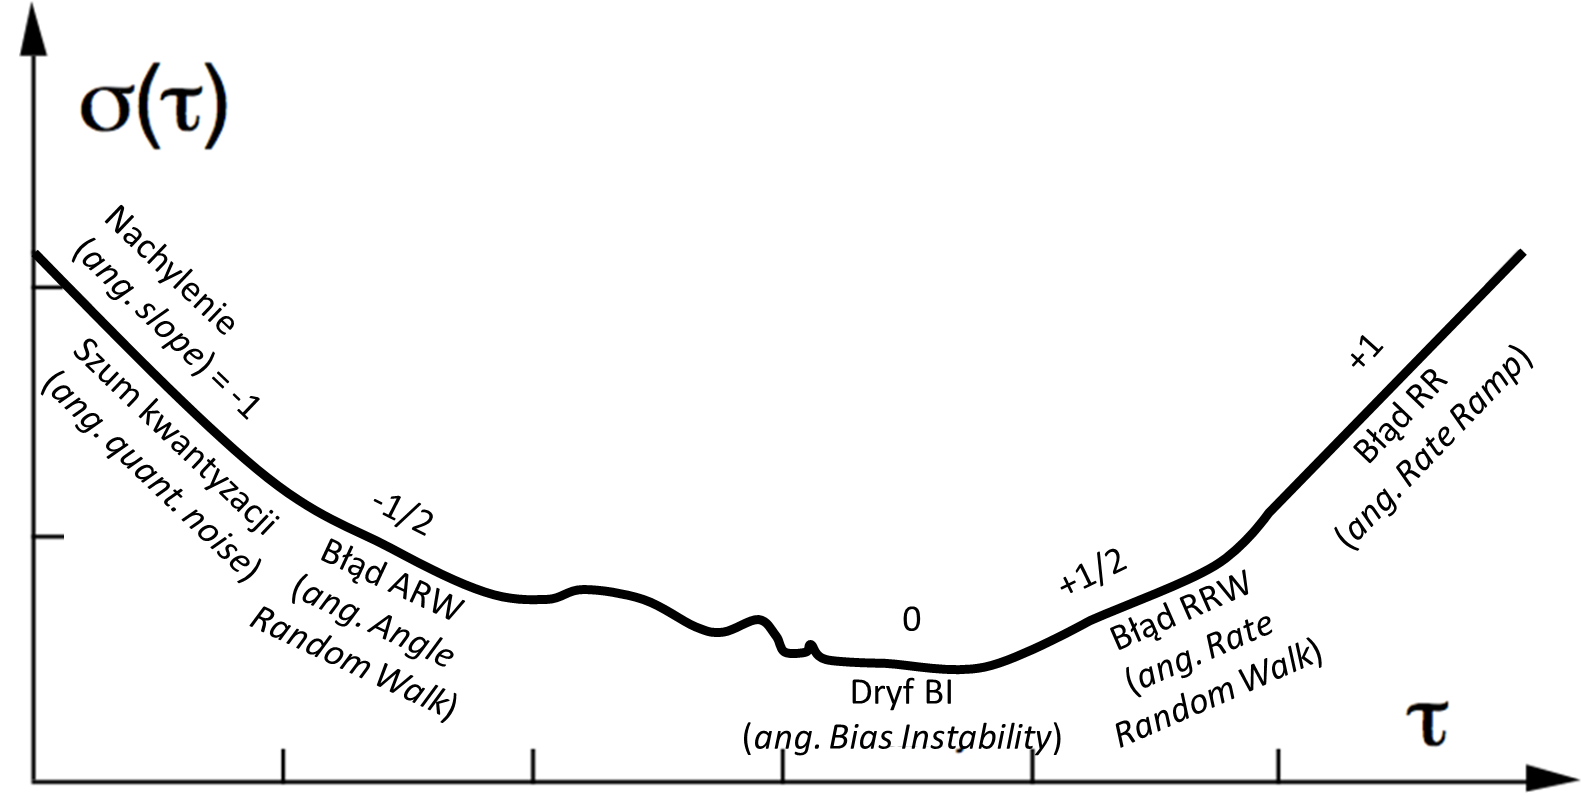
\includegraphics[width=\linewidth]{images/slopes.png}
		\caption[Obszary szumów na wykresie odchylenia Allana]{Obszary szumów na wykresie odchylenia Allana \cite{s120202219}}
		\label{fig:appx:allan:slopes}
	\end{figure}
\end{savenotes}
				
Nie zawsze wykres funkcji $\sigma(\tau)$ musi zawierać wszystkie 5 obszarów co oznacza, że niektóre rodzaje szumów mogą nie występować.